% =============================================================================
% Capitulo 4 - Implementación
% =============================================================================
\chapter{Implementación}
\label{cap:implementacion}

Este capítulo describe la implementación completa del sistema, desde la adquisición de la señal hasta el entrenamiento de los modelos. El sistema se organiza como un \emph{pipeline} en dos etapas (\emph{two-stage}): una primera etapa de detección y localización de ráfagas con YOLOv8 y una segunda etapa de clasificación del modelo de dron con ResNet18. Sobre esta arquitectura se describen además dos componentes de evaluación implementados: el clasificador de presencia a nivel de imagen, que traduce las detecciones geométricas de YOLO a una decisión operativa de hay dron o no hay dron, y el barrido de robustez frente a ruido, que cuantifica la degradación del sistema al contaminar la señal con distintos niveles de interferencia.


\section{Búsqueda y sintonía del canal del dron}

\subsection{Esquema de búsqueda}

Antes de iniciar la captura continua de muestras IQ es necesario un proceso previo de búsqueda en la banda de \SI{2.4}{\giga\hertz}, cuyo objetivo es localizar el canal en el que se estabiliza la transmisión del dron. Para ello se emplea un flujo de GNU Radio de exploración (\cref{fig:gnu_busqueda}) que visualiza el espectro en tiempo real y permite sintonizar manualmente la frecuencia central del receptor. En condiciones de baja interferencia la localización es sencilla, ya que la propia herramienta de visualización del espectro evidencia las transmisiones de alta potencia y las ráfagas características del enlace del dron. Cuando se observa una actividad compatible con un dron, se detiene el barrido y se extrae una captura breve de prueba para analizarla rápidamente y confirmar la presencia de la firma. Una vez identificada la frecuencia de la transmisión, se procede a la captura continua descrita en la \cref{sec:adquisicion_gnuradio}.

\begin{figure}[H]
    \centering
    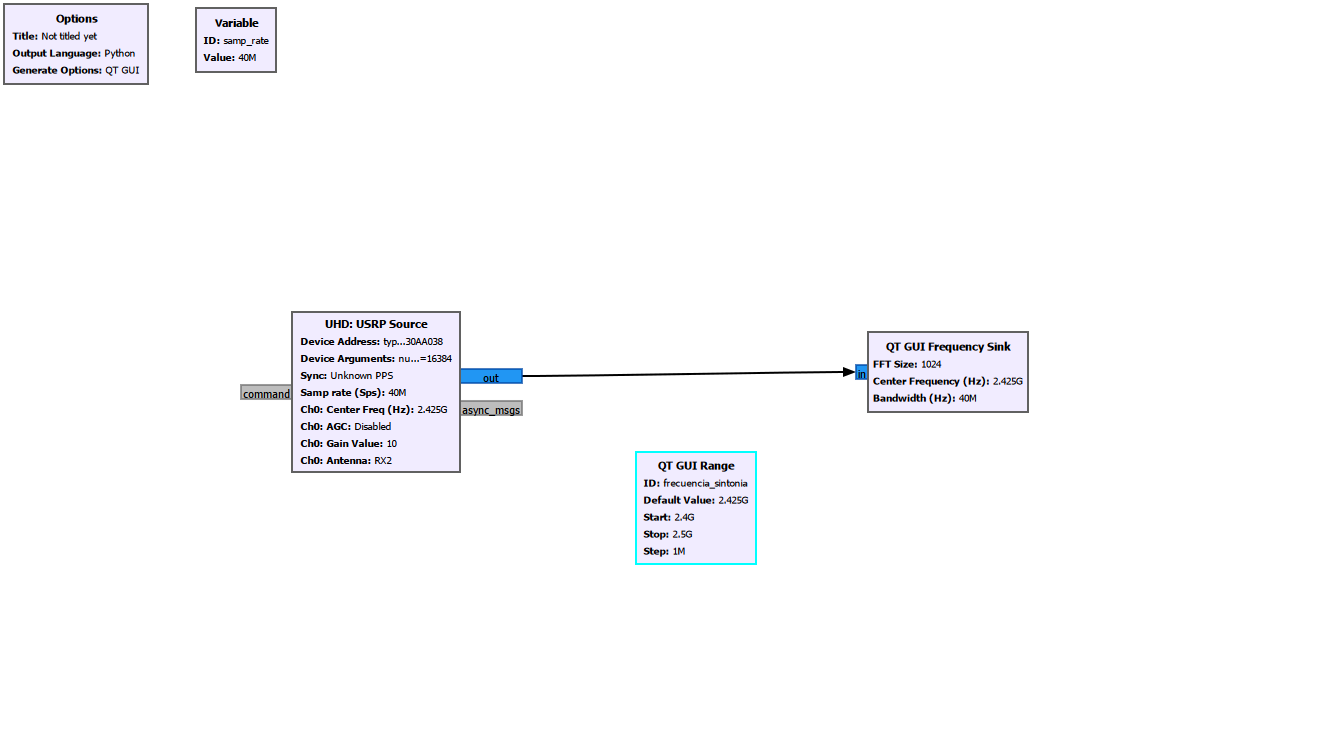
\includegraphics[width=0.95\textwidth]{figuras/implementacion/gnu_osci.png}
    \caption{Flujo de GNU Radio empleado en la fase de búsqueda y sintonía: el receptor USRP alimenta un visor de espectro en tiempo real cuya frecuencia central se controla mediante un deslizador que recorre la banda de \SI{2.4}{\giga\hertz}.}
    \label{fig:gnu_busqueda}
\end{figure}

El flujo de exploración consta de cuatro bloques principales. El bloque \texttt{UHD: USRP Source} configura el receptor: opera sobre el canal~0 con una frecuencia central sintonizable (valor por defecto \SI{2.425}{\giga\hertz}), una tasa de muestreo de \SI{40}{\mega\hertz}, ganancia fija de \num{10}, AGC desactivado y antena RX2. Su salida \texttt{out} se conecta directamente a un bloque \texttt{QT GUI Frequency Sink}, que calcula y muestra el espectro mediante una FFT de \num{1024} puntos sobre un ancho de banda de \SI{40}{\mega\hertz} centrado en la frecuencia sintonizada. Un bloque \texttt{QT GUI Range} (identificador \texttt{frecuencia\_sintonia}) genera un control deslizante que recorre el rango de \SIrange{2.4}{2.5}{\giga\hertz} con paso de \SI{1}{\mega\hertz} y se asocia a la frecuencia central del receptor, de modo que se puede desplazar la sintonía a lo largo de la banda en tiempo real. Finalmente, el bloque \texttt{Variable} fija la tasa de muestreo (\texttt{samp\_rate}~=~\SI{40}{\mega\hertz}) y el bloque \texttt{Options} define la generación del flujo en Python con interfaz QT GUI. A diferencia del flujo de captura, este flujo no almacena datos: su única función es la inspección visual del espectro para localizar la transmisión del dron.

\subsection{Búsqueda del dron en condiciones de alta congestión}

En escenarios de alta congestión RF la localización de la transmisión del dron se complica, ya que numerosos dispositivos WiFi y Bluetooth ocupan simultáneamente la banda. Para reproducir de forma controlada las condiciones más exigentes —las correspondientes al mayor número de dispositivos conectados— se fuerza manualmente al punto de acceso WiFi principal a operar en los canales bajos de la banda (canal~1, centrado en \SI{2412}{\mega\hertz}, o canal~6, en \SI{2437}{\mega\hertz}). Al concentrar la interferencia WiFi en la parte inferior del espectro, el mecanismo de salto de frecuencia adaptativo del enlace OcuSync~O2 tiende a desplazar sus ráfagas hacia la mitad superior de la banda de \SI{2.4}{\giga\hertz}, menos ocupada.

\vspace{1em}
Esta estrategia introduce inicialmente lo que parecía una limitación práctica. Con el ancho de banda instantáneo de \SI{40}{\mega\hertz} del receptor, una única ventana de observación no cubre la totalidad de la banda ISM (\SIrange{2400}{2483.5}{\mega\hertz}), por lo que no es posible centrar de forma perfecta la transmisión del dron: cuando el salto la sitúa cerca de los bordes del rango observado, algunas ráfagas aparecen incompletas o quedan fuera de la ventana. Para maximizar el número de transmisiones del dron efectivamente capturadas bajo interferencia forzada se sintonizaba la frecuencia central del receptor en \SI{2.46}{\giga\hertz}, de modo que la ventana de \SI{40}{\mega\hertz} (\SIrange{2440}{2480}{\mega\hertz}) abarcaba la mitad superior de la banda, donde se concentra la actividad del enlace en estas condiciones.

\vspace{1em}
Sin embargo, a lo largo del trabajo se constató que esa imposibilidad de centrar la señal no es realmente un inconveniente, sino una propiedad deseable para el entrenamiento del detector. En un despliegue real nunca se captura la transmisión del dron perfectamente centrada y aislada: son precisamente las interferencias del entorno las que fuerzan al enlace a aparecer en distintas posiciones y patrones dentro del espectrograma, manteniendo en todo momento sus rasgos morfológicos característicos —las ráfagas FHSS del enlace de mando y las franjas verticales de la transmisión de vídeo OFDM—. Esta variabilidad enriquece el conjunto de datos y permite que la red contraste un mayor número de situaciones. Por ello, en lugar de buscar una única condición ideal, se varió manualmente el canal del WiFi para forzar deliberadamente los saltos del dron y se realizaron medidas a lo largo de toda la banda de \SI{2.4}{\giga\hertz}, incorporando así escenarios marcadamente mixtos en los que las ráfagas del dron y las estructuras WiFi/Bluetooth coexisten en la misma ventana de observación, que son los casos más exigentes para el detector.

\section{Adquisición de señal en GNU Radio}
\label{sec:adquisicion_gnuradio}













\subsection{Estructura del flujo de captura}

El flujo de GNU Radio utilizado para la adquisición tiene una estructura sencilla:

\begin{center}
\texttt{UHD: USRP Source} $\rightarrow$ \texttt{Head} $\rightarrow$ \texttt{SigMF Sink}
\end{center}

El bloque \texttt{UHD: USRP Source} configura el receptor, la frecuencia central, la tasa de muestreo y la ganancia. El bloque \texttt{Head} limita el número de muestras para obtener capturas de duración controlada. Finalmente, el bloque \texttt{SigMF Sink} almacena los datos IQ junto con sus metadatos, permitiendo reproducir posteriormente las condiciones de adquisición.

\subsection{Variables globales}

Las variables principales del flujo son la frecuencia central, la tasa de muestreo, la ganancia y la duración de captura. La campaña utiliza una tasa de muestreo fija $f_s = \SI{40}{\mega\hertz}$ y una ganancia fija de \num{10} con el control automático de ganancia (AGC) desactivado, de modo que el nivel de señal no introduce un sesgo de ganancia entre capturas. Para capturar una duración $T$ con una tasa de muestreo $f_s$, el número de muestras complejas que debe dejar pasar el bloque \texttt{Head} es:

\begin{equation}
N = f_s\, T.
\end{equation}

Por ejemplo, una captura efectiva de \SI{15}{\second} a \SI{40}{\mega\hertz} requiere \num{600e6} muestras complejas, que posteriormente se segmentan en \num{150} espectrogramas de \SI{0.1}{\second}. Fijar $f_s$ y la duración garantiza capturas comparables entre escenarios.

\subsection{Almacenamiento SigMF}

El formato SigMF separa los datos IQ binarios (\texttt{.sigmf-data}) del fichero de metadatos (\texttt{.sigmf-meta}). Esta estructura resulta útil para el TFG porque conserva la información de frecuencia central, tasa de muestreo y formato de muestra. Los scripts de Python leen estos metadatos para reconstruir correctamente el eje de frecuencia absoluta de cada espectrograma, sin asumir valores fijos en el código.




\subsection{Montaje experimental}
\label{sec:montaje_experimental}

El montaje de captura está formado por tres elementos: la antena receptora, el receptor SDR y la fuente de señal. La antena se conecta directamente al USRP B210, conectado por USB 3.0 al equipo de adquisición, que se controla mediante GNU Radio en ejecución. Este receptor permite obtener muestras IQ complejas con un ancho de banda suficiente para observar las estructuras de transmisión de la banda ISM de \SI{2.4}{\giga\hertz}, y almacena las muestras en formato SigMF para su posterior procesado. La configuración de adquisición (antena directional fija, ganancia constante, AGC desactivado y tasa de muestreo de \SI{40}{\mega\hertz}) se mantiene idéntica en los dos tipos de captura, de modo que la única diferencia entre ellos es la fuente de señal presente.

\subsubsection{Captura de dron}

Previamente a capturar los datos IQ recibidos por la antena hay que hacer un trabajo de búsqueda porla banda de 2.4GHz, en la cual nuestro objetivo será encontrar el canal en el que se ha estabilizado la transmisión del dron. Cuando hay pocas interferencias alrededor del dron no es difícil encontrarlo, principalmente por la propia herramienta de visualización de espectro que hemos configurado en GNU radio, en la cual cuando sospechamos que aparecen transmisiones de mucha potencia o burst que nos hagan sospechar que puede haber un dron lo que hacemos es parar la búsqueda y sacamos un archivo de prueba para analizarlo rapidamente. Todo esto es un proceso previo a la captura de datos de manera continua es para encontrar la trasmision




En las capturas de dron, la fuente de señal de interés es el propio dron, que permanece encendido con su enlace de comunicación activo, de modo que sus ráfagas FHSS quedan dentro del lóbulo de la antena directional orientada hacia él. La \cref{fig:setup_antena} ilustra el montaje físico de este tipo de medida. El dron se captura sobre el fondo WiFi del entorno presente durante la campaña, en los niveles de congestión definidos en la \cref{tab:niveles_interferencia}: el objetivo es caracterizar y encontrar la firma del dron como emisor dominante, antes de pasar al escenario mixto con interferencia saturada. 

Una vez confirmamos la presencia del dron gracias a nuestra búsqueda por oscilos

\begin{figure}[H]
    \centering
    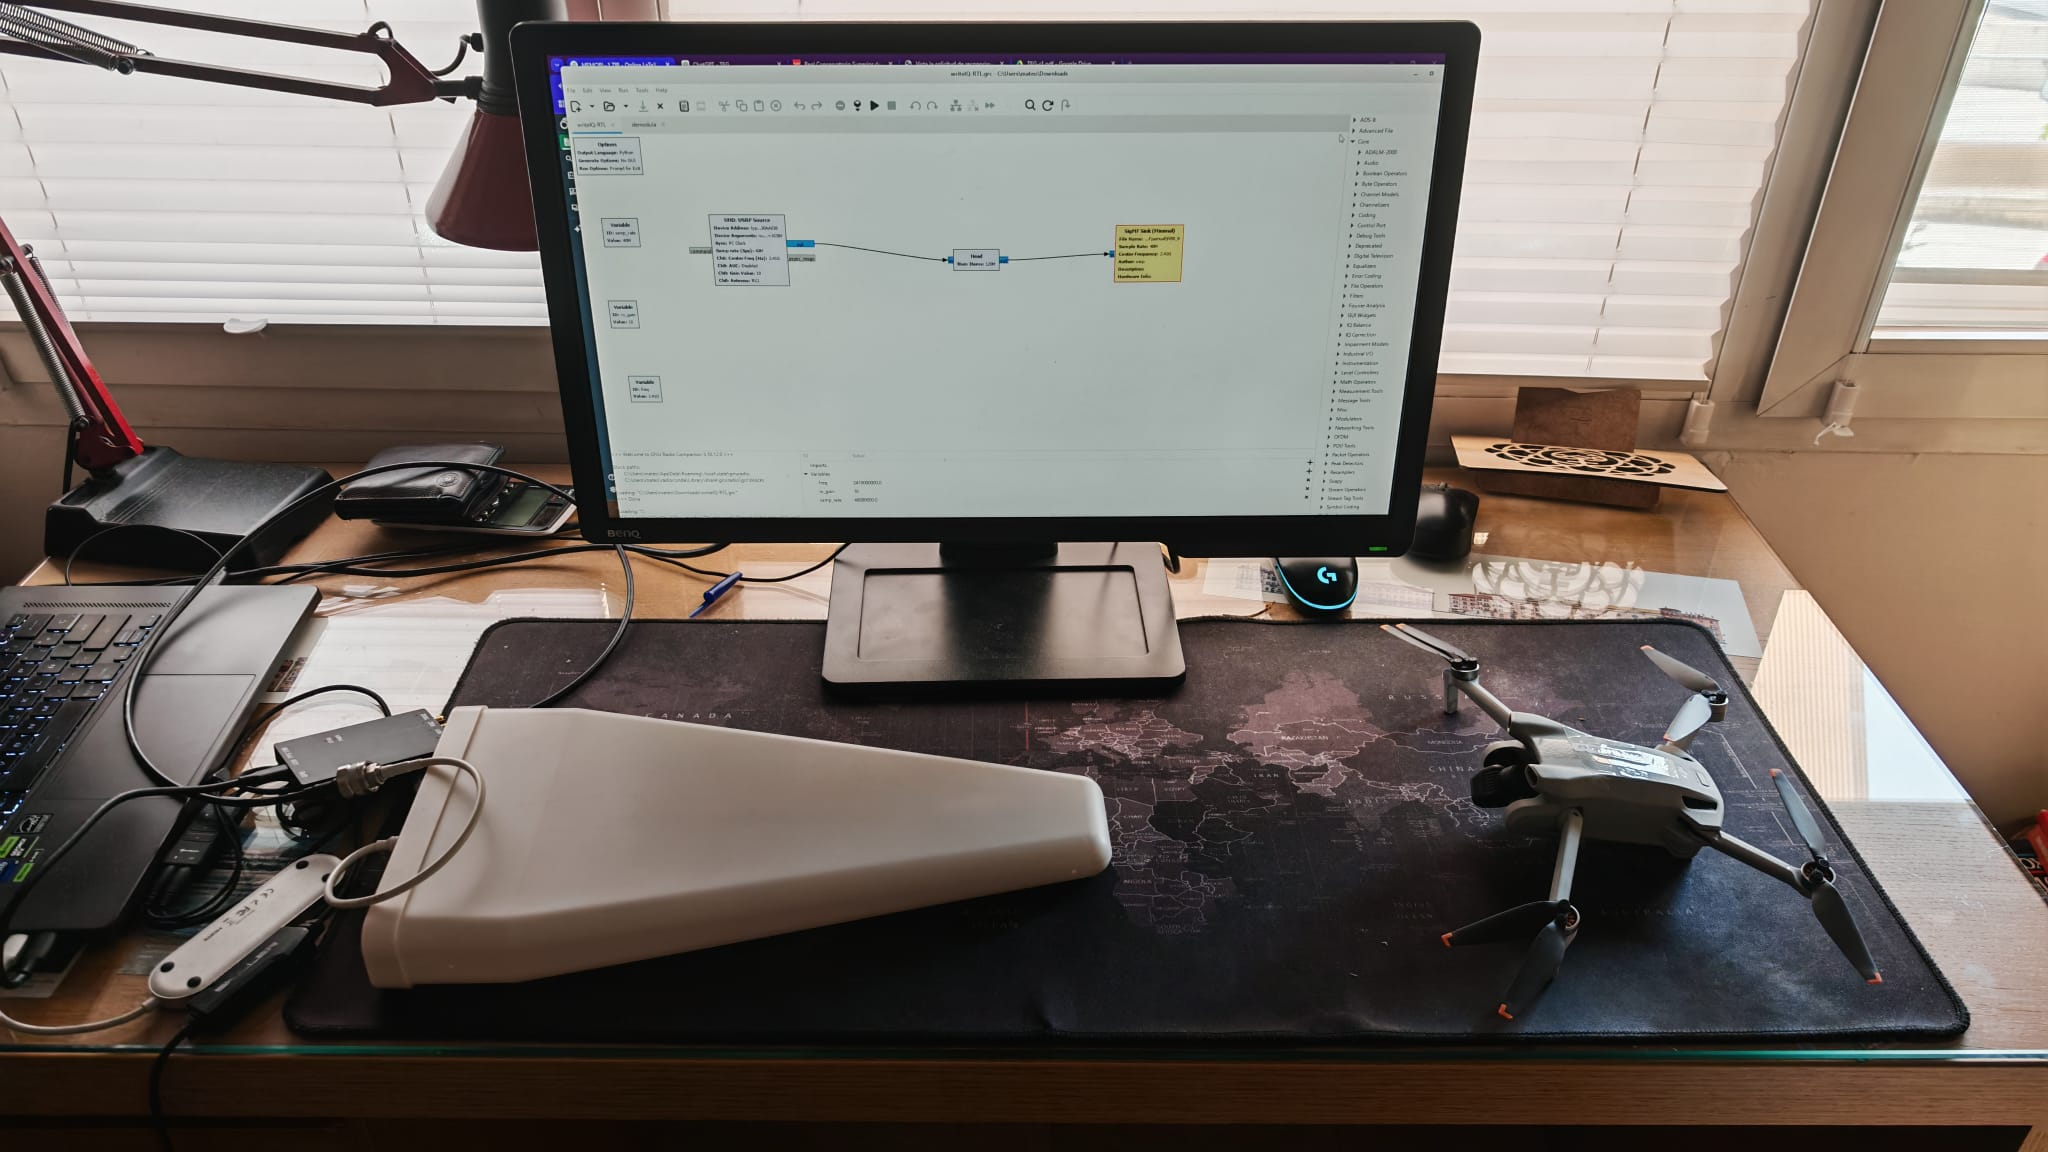
\includegraphics[width=0.85\textwidth]{figuras/implementacion/esquema.jpeg}
    \caption{Montaje experimental para la captura de dron: antena receptora conectada al USRP con GNU Radio en ejecución y el dron como fuente de señal dominante.}
    \label{fig:setup_antena}
\end{figure}

\subsubsection{Captura de interferencia}

En las capturas de interferencia se mantiene exactamente el mismo montaje (antena, posición, ganancia y receptor), pero con el dron apagado. La señal presente procede únicamente de las fuentes de interferencia del entorno, principalmente tráfico WiFi en la banda de \SI{2.4}{\giga\hertz} y, en algunos casos, Bluetooth. Para que la interferencia se reciba con potencia suficiente, los puntos de acceso WiFi se sitúan dentro del lóbulo de la antena directional. Estas capturas se realizan con distintos niveles de congestión para estudiar su efecto, desde tráfico ligero hasta saturación de la banda. Para generar distintos niveles de tráfico WiFi se emplean tanto ordenadores como teléfonos móviles realizando descargas, videollamadas, navegación por internet o vídeo en streaming. Para el Bluetooth se utilizan auriculares, mandos de consola y ratones inalámbricos, que producen ráfagas repartidas en frecuencia con una morfología similar a la del enlace del dron.


Las capturas de interferencia no se realizan en una única condición, sino en tres niveles de congestión creciente de la banda de \SI{2.4}{\giga\hertz}. El objetivo es estudiar cómo afecta la cantidad de tráfico al problema de clasificación, generando la interferencia de forma activa con dispositivos reales para que la ocupación de la banda sea representativa. Los tres niveles se definen aumentando progresivamente el número de fuentes y la intensidad del tráfico:

\begin{itemize}
  \item \textbf{Nivel W1 (bajo):} interferencia ligera. Uno o varios dispositivos reproduciendo vídeo en streaming y un único dispositivo Bluetooth activo o ninguno.
  \item \textbf{Nivel W2 (moderado):} un dispositivo generando tráfico intenso de descarga junto con más de un dispositivo Bluetooth activo.
  \item \textbf{Nivel W3 (alto):} varios dispositivos en descarga y videollamada simultáneas, junto con varios dispositivos Bluetooth activos, saturando la banda.
\end{itemize}

\begin{table}[H]
\centering
\caption{Definición de los tres niveles de interferencia empleados en las capturas.}
\label{tab:niveles_interferencia}
\begin{tabular}{cll}
\toprule
\textbf{Nivel} & \textbf{Tráfico WiFi} & \textbf{Bluetooth} \\
\midrule
W1 & Video streaming & 1 dispositivo \\
W2 & Descarga de alto tráfico & $>$1 dispositivo \\
W3 & Varias descargas + videollamada & Varios dispositivos \\
\bottomrule
\end{tabular}
\end{table}

La inclusión de dispositivos Bluetooth en todos los niveles es deliberada: el Bluetooth también usa saltos de frecuencia (FHSS) con ráfagas de morfología similar a las del dron, por lo que aumenta la dificultad del problema y acerca las capturas al escenario real. El número creciente de fuentes Bluetooth entre W1 y W3 incrementa esa dificultad de forma controlada.

\subsubsection{Captura de entorno mixto}

Las capturas de entorno mixto combinan las dos fuentes anteriores: el dron encendido y, de forma simultánea, las fuentes de interferencia WiFi activas en niveles de congestión altos. Reproducen el escenario realista de despliegue, en el que la señal del dron debe distinguirse en presencia de un fondo RF saturado. El montaje es de nuevo idéntico al de los otros dos casos. 





\begin{figure}[H]
    \centering
    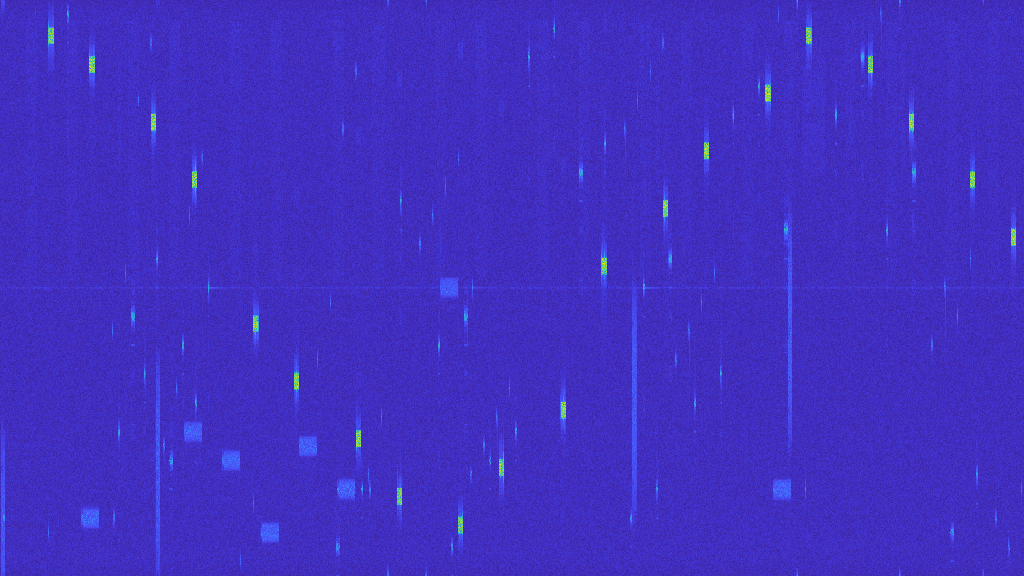
\includegraphics[width=0.85\textwidth]{figuras/implementacion/dronmixto.png}
    \caption{Montaje experimental para la captura en entorno mixto: el dron encendido y las fuentes de interferencia WiFi activas de forma simultánea, reproduciendo el escenario realista de despliegue con fondo RF saturado.}
    \label{fig:setup_mixto}
\end{figure}









\section{Generación de espectrogramas}
\label{sec:generacion_espectrogramas}

La generación de espectrogramas la realiza el script \texttt{make\_spectrogram\_dataset.py}, que convierte cada fichero SigMF en un conjunto de imágenes PNG y registra los metadatos en un CSV maestro.

\subsection{Lectura por segmentos}

Cada fichero SigMF se lee por bloques temporales de \SI{0.1}{\second}. Esta ventana se selecciona porque ofrece un compromiso práctico: es suficientemente corta para generar muchos ejemplos por captura y suficientemente larga para observar patrones de ráfagas y saltos de frecuencia. El número de muestras por segmento es $f_s \cdot \SI{0.1}{\second} = \num{4e6}$ muestras complejas. Cada segmento se lee de forma independiente mediante un acceso por desplazamiento de bytes sobre el fichero binario, sin cargar la captura completa en memoria, y se libera explícitamente la memoria entre segmentos para limitar el consumo de RAM.


\begin{figure}[H]
    \centering
    \begin{subfigure}[b]{0.48\textwidth}
        \centering
        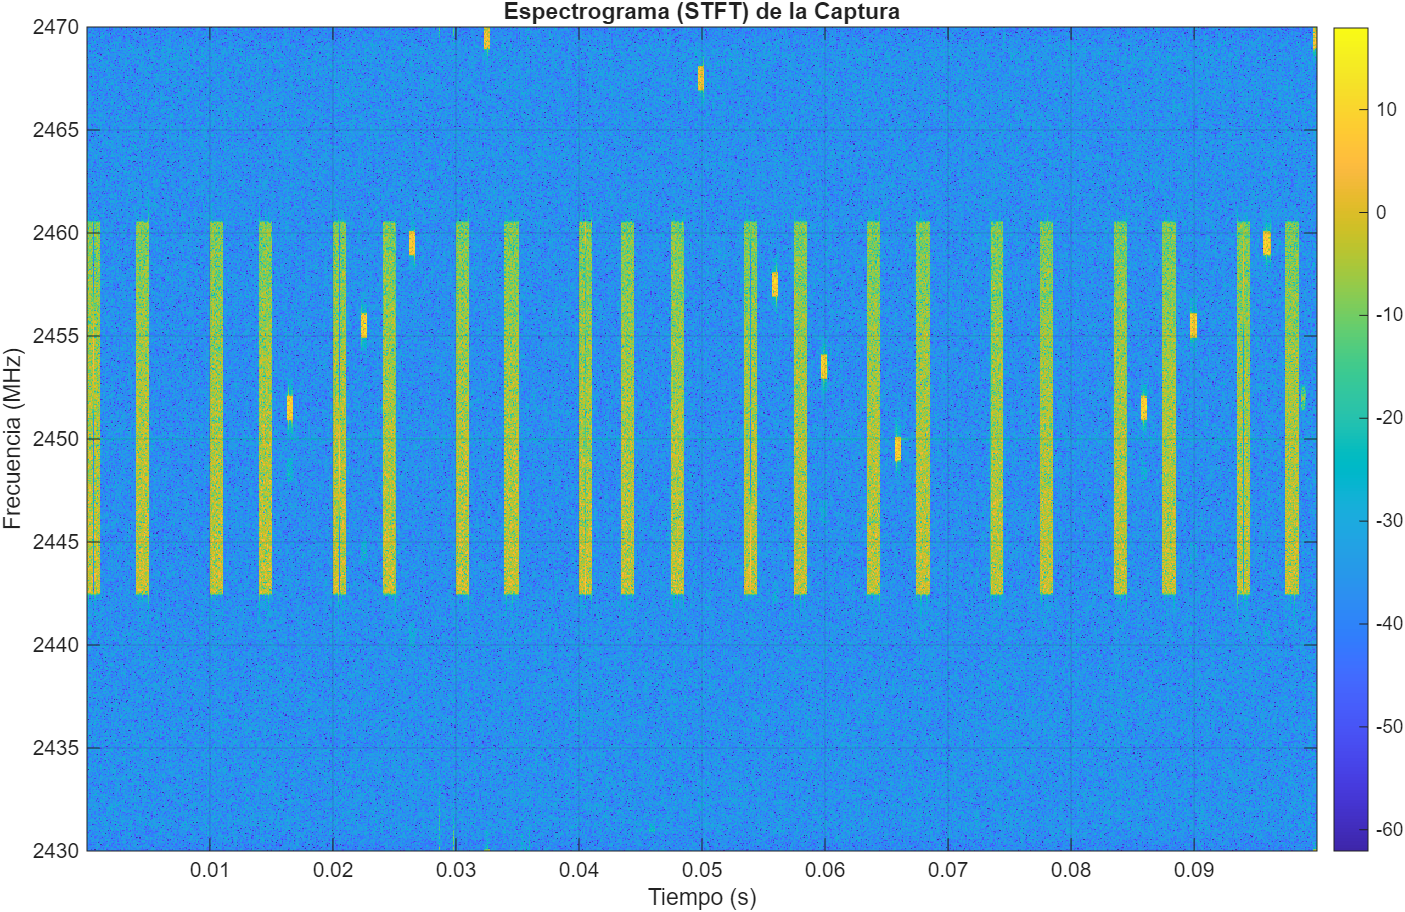
\includegraphics[width=\textwidth]{figuras/requisitos/dron_0_1s.png}
        \caption{Ventana de \SI{0.1}{\second}.}
        \label{fig:espectro_01s}
    \end{subfigure}
    \hfill
    \begin{subfigure}[b]{0.48\textwidth}
        \centering
        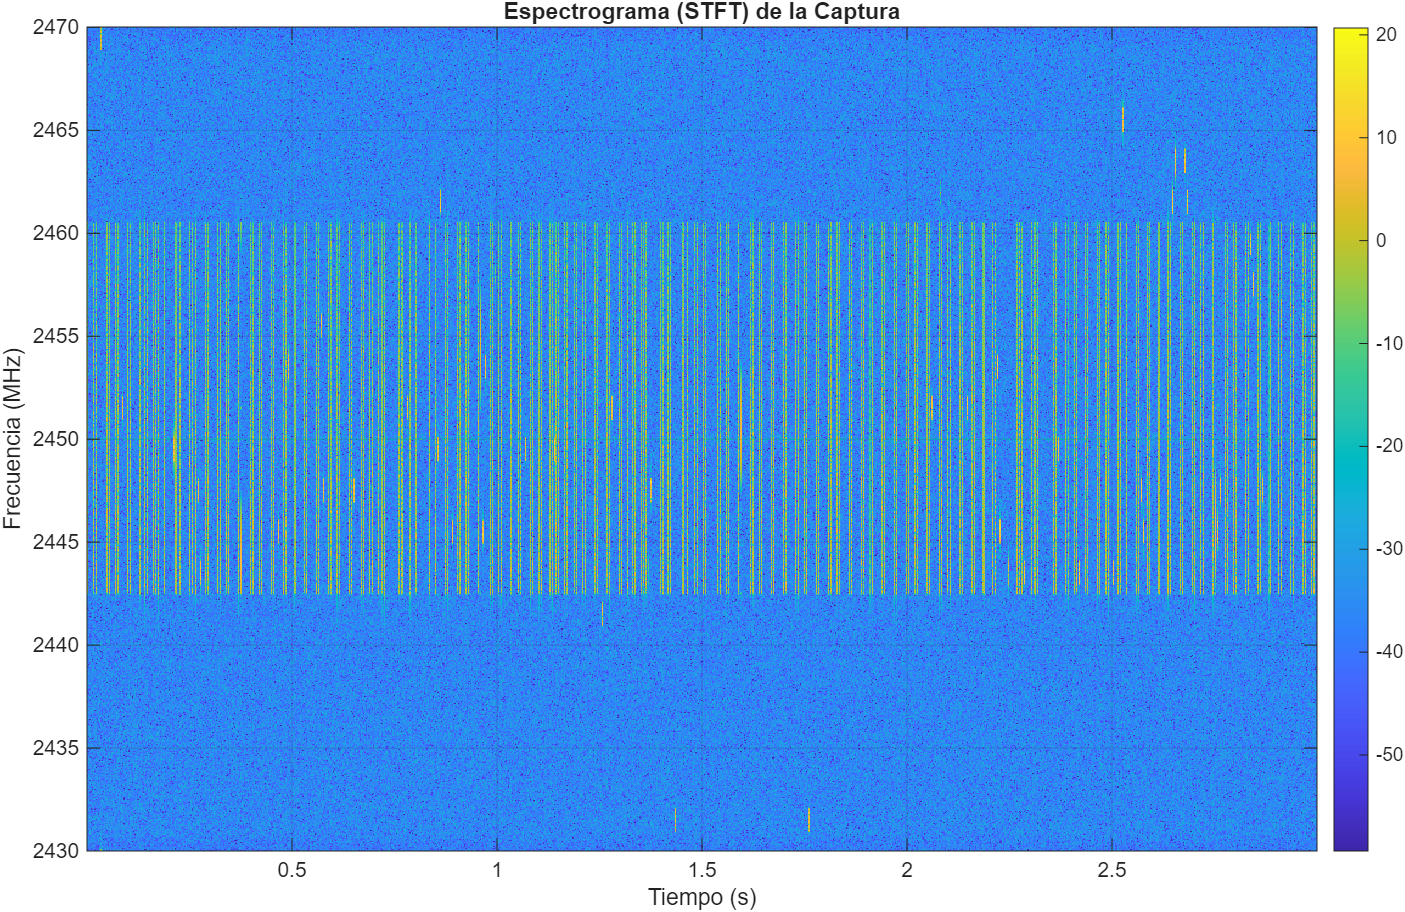
\includegraphics[width=\textwidth]{figuras/requisitos/dron_segundos.png}
        \caption{Ventana de \SI{3}{\second}.}
        \label{fig:espectro_3s}
    \end{subfigure}
    \caption{Comparación de la transmisión del DJI Mini 3 representada con dos ventanas temporales. La ventana corta de \SI{0.1}{\second} (a) resuelve las ráfagas FHSS individuales, mientras que la ventana larga de \SI{3}{\second} (b) las acumula y dificulta distinguir su morfología.}
    \label{fig:comparacion_ventanas}
\end{figure}
\subsection{Cálculo de la STFT}

La representación tiempo-frecuencia se calcula mediante la transformada de Fourier de tiempo corto. Para una señal discreta $x[n]$, la STFT se define como:

\begin{equation}
X(m,k)=\sum_n x[n]\,w[n-mH]\,e^{-j2\pi kn/N},
\end{equation}

donde $w[n]$ es la ventana de análisis, $H$ es el salto entre ventanas, $N$ es el número de puntos de la FFT y $k$ es el índice frecuencial. En la implementación se utiliza una ventana de Hann periódica con $N = \num{1024}$ puntos y un solapamiento del \SI{75}{\percent} ($\num{768}$ muestras). Se calcula el espectro completo de doble banda y se aplica \texttt{fftshift} para centrar la componente de continua, emulando el modo \emph{centered}. Estos parámetros son idénticos en entrenamiento, validación y prueba.

De la STFT se derivan dos resoluciones que determinan el detalle del espectrograma. La \emph{resolución frecuencial} $\Delta f$ es la separación mínima en frecuencia que se puede distinguir, es decir, la anchura de cada bin de la FFT. La \emph{resolución temporal} $\Delta t$ es el intervalo de tiempo más corto que se puede resolver, ligado a la duración de la ventana de análisis. Ambas dependen del número de puntos de la FFT, $N$, y de la tasa de muestreo, $f_s$:

\begin{equation}
\Delta f = \frac{f_s}{N} \approx \SI{39}{\kilo\hertz}, \qquad
\Delta t = \frac{N}{f_s} \approx \SI{25.6}{\micro\second}.
\end{equation}

Existe un compromiso entre ambas: al aumentar $N$ mejora la resolución frecuencial (bins más estrechos) pero empeora la temporal (ventanas más largas), y viceversa. La elección de $N = \num{1024}$ equilibra las dos: ofrece una resolución frecuencial de unos \SI{39}{\kilo\hertz} y una resolución temporal de unos \SI{25.6}{\micro\second}, suficiente para resolver ráfagas FHSS de \SIrange{100}{500}{\micro\second} como las de la señal del dron o del Bluetooth, así como la estructura interna de las tramas WiFi.

La potencia se expresa en decibelios mediante:

\begin{equation}
P_{\mathrm{dB}} = 10\log_{10}\left(|X(m,k)|^2 + \epsilon\right),
\end{equation}

donde $\epsilon$ evita problemas numéricos al tomar el logaritmo de valores cercanos a cero. El eje de frecuencia se expresa en valor absoluto mediante $F_{\mathrm{abs}} = (F + f_c)/10^6$ en MHz, usando la frecuencia central $f_c$ leída de los metadatos SigMF.


El cálculo se implementa con \texttt{scipy.signal.spectrogram}, manteniendo los parámetros descritos:

\begin{lstlisting}[style=python,caption={Cálculo de la STFT de cada segmento.}]
win = windows.hann(NFFT, sym=False)      # Hann periodica, NFFT = 1024
overlap = round(0.75 * NFFT)             # solape del 75%

F, T, S = spectrogram(senal_seg, fs=fs, window=win,
                      nperseg=NFFT, noverlap=overlap, nfft=NFFT,
                      return_onesided=False, mode="complex")

F = np.fft.fftshift(F)                   # centrar la componente de continua
S = np.fft.fftshift(S, axes=0)

Pdb = 10 * np.log10(np.abs(S)**2 + eps)  # potencia en dB
\end{lstlisting}


\subsection{Renderizado y exportación}

Cada espectrograma se exporta como imagen PNG de \num{1024}x\num{576} píxeles a \num{120} ppp usando el mapa de color Parula. La escala de color es automática por imagen, fijada al rango $[\,\text{max}_{\mathrm{dB}} - \SI{80}{\decibel},\ \text{max}_{\mathrm{dB}}\,]$. Mantener el mismo procedimiento de renderizado en todas las particiones asegura que las diferencias aprendidas por el modelo procedan de la señal y no de cambios en la visualización.




\subsection{CSV maestro}

El script genera de forma incremental un CSV maestro con una fila por espectrograma. Las columnas registran el nombre de fichero, la etiqueta, el nivel WiFi, la condición (limpia o mixta), la antena, la distancia, el entorno, la frecuencia central, la tasa de muestreo, la ganancia, el identificador de captura y la plataforma. Estos metadatos permiten construir los splits y analizar resultados por subgrupos.


\subsection{Ejemplo de espectrograma generado}
\label{sec:ejemplo_espectrograma}

La \cref{fig:salto_frecuencia} muestra un espectrograma generado con el procedimiento descrito. En él se aprecia de forma directa el comportamiento de salto de frecuencia de OcuSync: a lo largo de la ventana de \SI{0.1}{\second}, las ráfagas del enlace del dron (regiones brillantes) no se mantienen en una frecuencia fija, sino que se reubican en distintos puntos del espectro, ocupando los huecos libres dentro de la banda de \SI{2.4}{\giga\hertz} y evitando las zonas ocupadas por el WiFi. Las columnas verticales más anchas y tenues corresponden a la ocupación más estable de las señales WiFi, de canal fijo. Cada ráfaga corresponde a una transmisión OFDM del enlace de vídeo, cuya frecuencia central varía de un salto al siguiente. Este patrón es precisamente la firma morfológica que el detector debe aprender a distinguir.

\begin{figure}[H]
    \centering
    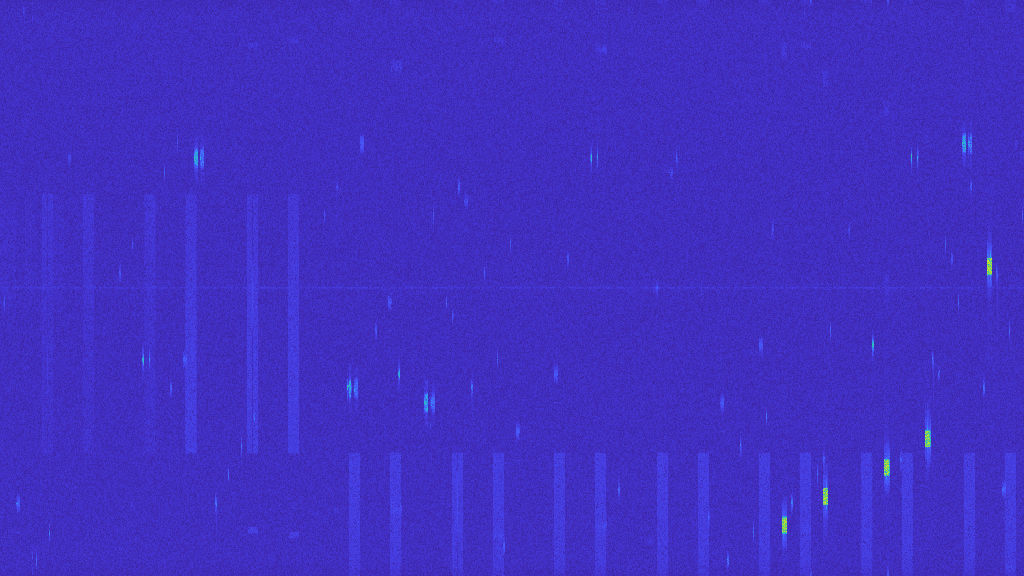
\includegraphics[width=0.9\textwidth]{figuras/implementacion/cambiofrec.png}
    \caption{Espectrograma de \SI{0.1}{\second} generado a partir de una captura del DJI Mini 3. Se observa el salto de frecuencia adaptativo de OcuSync: las ráfagas del enlace del dron aparecen a distintas frecuencias a lo largo de la ventana temporal, mientras que las columnas verticales más anchas y estables corresponden a la actividad WiFi.}
    \label{fig:salto_frecuencia}
\end{figure}





\section{Preparación del dataset YOLO}
\label{sec:preparacion_yolo}

\subsection{Estructura de carpetas}

El dataset para YOLO se organiza en imágenes y etiquetas. Cada imagen PNG tiene asociado un fichero \texttt{.txt} con las cajas delimitadoras en formato YOLO:

\begin{lstlisting}[caption={Formato de una etiqueta YOLO.}]
<class_id> <x_center> <y_center> <width> <height>
\end{lstlisting}

Las coordenadas se normalizan respecto al ancho y alto de la imagen. Las clases utilizadas son \texttt{interference} (clase 0) y \texttt{drone} (clase 1). Además, se genera un fichero \texttt{data.yaml} que define las rutas de entrenamiento, validación y prueba, así como el número y nombre de las clases.




\subsection{Partición por captura}

La partición se realiza con el script \texttt{split\_capture\_level.py} a nivel de captura completa, con proporciones objetivo aproximadas de \num{70}/\num{15}/\num{15} para entrenamiento, validación y prueba, estratificando por etiqueta y con semilla fija \num{42}. Como la partición es por captura entera y no por imagen, el reparto efectivo de espectrogramas no cae exactamente sobre esas proporciones. Este punto es esencial porque los espectrogramas consecutivos de una misma captura comparten condiciones de canal, ganancia, distancia, entorno e interferencias. Si se mezclasen segmentos de una misma captura entre entrenamiento y prueba, la evaluación estaría sesgada por fuga de información. El script incluye una comprobación de no solapamiento que aborta el proceso si algún identificador de captura aparece en más de una partición. No se copian las imágenes entre carpetas: los splits se materializan como listas de rutas relativas.

\section{Auto-etiquetado de ráfagas}
\label{sec:autoetiquetado}

El script \texttt{auto\_label\_bursts.py} genera automáticamente cajas delimitadoras sobre los espectrogramas. El procedimiento se resume en los siguientes pasos:

\begin{enumerate}
  \item leer la imagen del espectrograma;
  \item convertirla a una representación de intensidad y aplicar un suavizado mínimo;
  \item aplicar un umbral en el percentil \num{99.8};
  \item encontrar componentes conectados;
  \item descartar regiones demasiado pequeñas o demasiado grandes;
  \item convertir las cajas al formato YOLO normalizado;
  \item asignar la clase en función de la captura de origen.
\end{enumerate}

La calibración final utiliza un umbral en el percentil \num{99.8}, un área mínima de \num{8} píxeles, un área máxima del \num{0.005} de la imagen, un núcleo morfológico de tamaño \num{1} (sin operación morfológica, para preservar blobs sueltos) y un suavizado gaussiano de $\sigma = \num{0.4}$. Estos valores surgen de un proceso iterativo: las primeras calibraciones (percentil \num{99}, área mínima de \num{200} píxeles, núcleo de tamaño \num{5}) capturaban barras WiFi enteras y las etiquetaban incorrectamente. El filtro final descarta de forma implícita las barras WiFi anchas, que ocupan áreas mucho mayores, y conserva ráfagas FHSS pequeñas compatibles con OcuSync o Bluetooth.

La \cref{fig:yolo_cajas} muestra un ejemplo de espectrograma con sus cajas delimitadoras. Cada caja (en rojo) encierra una ráfaga individual, que es el objeto que el detector debe localizar y clasificar. Obsérvese que las columnas verticales anchas, correspondientes a la actividad WiFi de canal fijo, no quedan enmarcadas: el criterio de área máxima del auto-etiquetado las descarta por su tamaño, de modo que las etiquetas se concentran exclusivamente en las ráfagas estrechas de salto de frecuencia. Esta es precisamente la diferencia frente a un clasificador de imagen completa: al trabajar sobre regiones locales, el modelo atiende a la morfología de cada ráfaga y no al contexto global de la captura.

\begin{figure}[H]
    \centering
    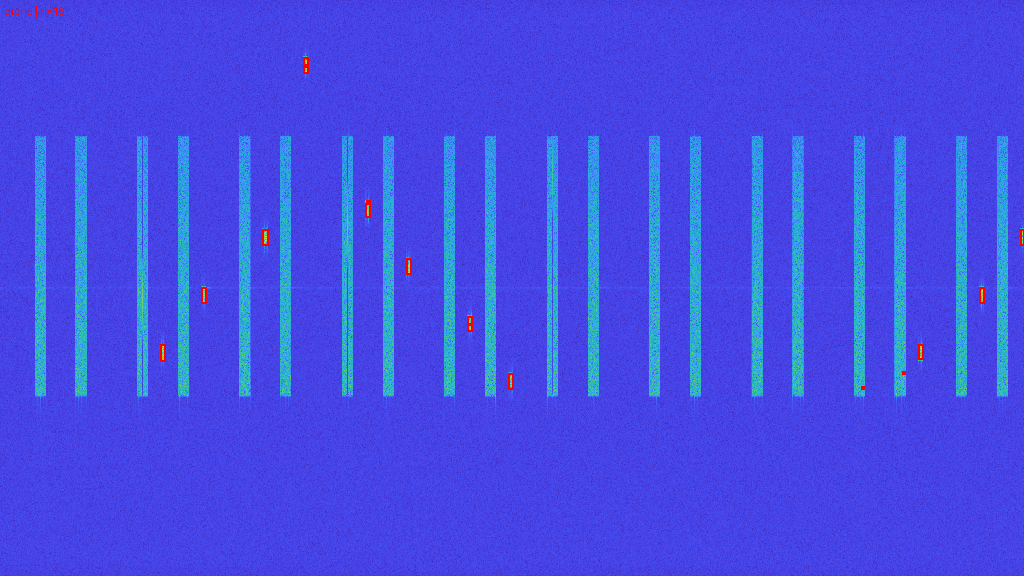
\includegraphics[width=0.9\textwidth]{figuras/implementacion/preview.png}
    \caption{Ejemplo de espectrograma con las cajas delimitadoras en formato YOLO para una captura limpia de dron.}
    \label{fig:yolo_cajas}
\end{figure}


\begin{figure}[H]
    \centering
    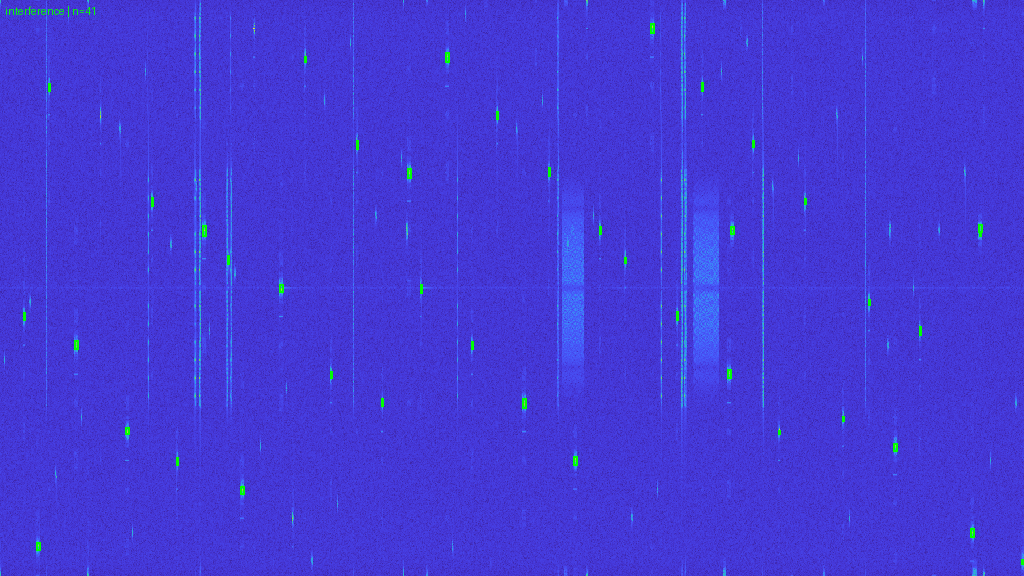
\includegraphics[width=0.9\textwidth]{figuras/implementacion/preview_interference.png}
    \caption{Ejemplo de espectrograma con las cajas delimitadoras en formato YOLO para una captura de interferencia.}
    \label{fig:yolo_cajas_interference}
\end{figure}


La \cref{fig:yolo_cajas_interference} muestra el mismo procedimiento aplicado a una captura sin dron. En este caso, las cajas no se asocian al enlace del dron, sino a las ráfagas dispersas procedentes de Bluetooth y de otras emisiones ISM residuales, que aparecen como pequeños segmentos repartidos por toda la banda y que el auto-etiquetado marca como clase \emph{interference}. Al igual que en la captura de dron, las estructuras verticales más anchas y tenues —atribuibles a la actividad WiFi de canal fijo— quedan descartadas por el criterio de área máxima y no se enmarcan.  La etiqueta \texttt{n=41} indica el número de regiones detectadas en este segmento, evidenciando la densidad de emisores activos en la banda durante la captura.


\subsection{Etiquetado débil y su justificación}

La clase de cada caja se hereda de la captura de origen: las cajas de capturas \texttt{mini3\_drone\_*} se etiquetan como \texttt{drone} y las de capturas \texttt{mini3\_nodrone\_*} como \texttt{interference}. Se trata de un etiquetado débil, pero coherente con el diseño de la campaña: en las capturas de dron no se añaden fuentes Bluetooth dedicadas, por lo que el dron es la fuente FHSS dominante frente al fondo WiFi del entorno, mientras que las capturas sin dron sí incorporan Bluetooth, de modo que las ráfagas detectadas en ellas corresponden a interferencia y no al enlace OcuSync O2. 

\vspace{1em}
Esta coherencia permite entrenar un detector sin anotación manual exhaustiva. No obstante, al asignar la clase por captura completa toda ráfaga de una captura de dron se etiqueta como \texttt{drone} aunque parte de la energía proceda del fondo WiFi, lo que introduce un ruido de etiquetado que se asume como limitación documentada del procedimiento.

\begin{lstlisting}[style=python,caption={Pseudocódigo del auto-etiquetado de ráfagas.}]
img = read_spectrogram(path)
intensity = smooth(to_intensity(img), sigma=0.4)
mask = intensity > percentile(intensity, 99.8)
components = connected_components(mask)

for comp in components:
    box = bounding_box(comp)
    area = box.width * box.height
    if area < min_area_px:            # min_area_px = 8
        continue
    if area > max_area_frac * image_area:   # max_area_frac = 0.005
        continue
    write_yolo_label(box, class_from_capture(path))
\end{lstlisting}





La razón de que el auto-etiquetado conserve únicamente las ráfagas pequeñas, descartando las columnas anchas del WiFi, es metodológica. Distinguir el dron de una señal WiFi es un problema trivial: el WiFi se manifiesta como columnas verticales anchas y fijas, fácilmente separables de cualquier ráfaga de salto de frecuencia mediante descriptores elementales. Un detector que resolviera únicamente esa distinción no demostraría haber aprendido la firma del dron.

El problema científicamente relevante es separar la firma FHSS de OcuSync de otras señales de salto de frecuencia presentes en la banda, en particular del Bluetooth, que comparte con el dron la técnica FHSS y una morfología de ráfagas estrechas y dispersas muy similar. Al filtrar implícitamente las barras WiFi por su tamaño, las ráfagas conservadas en las capturas sin dron corresponden mayoritariamente a Bluetooth. De este modo, la tarea de detección enfrenta dos señales de morfología parecida, y un resultado positivo del modelo evidencia que ha aprendido las diferencias finas entre ambas (ancho de banda por ráfaga, duración y patrón de salto) y no un atajo trivial frente al WiFi. Esto convierte el problema en un banco de pruebas mucho más exigente y representativo del escenario real.

Conviene matizar el papel que desempeña el WiFi en este planteamiento. Aunque sus barras anchas se descartan en el etiquetado y no constituyen la clase que el detector debe separar del dron, la actividad WiFi no es prescindible: su utilidad principal es actuar como agente perturbador del entorno. Por un lado, degrada la calidad de la señal recibida del dron al elevar el nivel de ocupación y de ruido en la banda, reduciendo la relación señal a ruido de sus ráfagas. Por otro, y de forma más determinante, fuerza el mecanismo de salto de frecuencia adaptativo del enlace OcuSync~O2 a reubicar sus transmisiones en los huecos libres del espectro, modificando dinámicamente la posición y el patrón de las ráfagas del dron. De este modo, el WiFi no se trata como una clase a discriminar, sino como el elemento que genera la diversidad de condiciones —distintas posiciones, niveles de potencia y grados de solapamiento— sobre las que el detector debe demostrar que reconoce la firma del dron.


\section{Entrenamiento del detector YOLOv8 (Stage 1)}
\label{sec:entrenamiento_yolo}

El entrenamiento se realiza con YOLOv8n, una variante ligera de aproximadamente tres millones de parámetros. Se parte de pesos preentrenados en COCO y se ajusta el modelo al dataset de espectrogramas mediante \texttt{train\_yolo.py}, un envoltorio sobre Ultralytics. La configuración principal es:

\begin{table}[htbp]
\centering
\caption{Configuración principal del entrenamiento YOLOv8n.}
\label{tab:config_yolo}
\begin{tabular}{ll}
\toprule
\textbf{Parámetro} & \textbf{Valor} \\
\midrule
Modelo base & \texttt{yolov8n.pt} \\
Tamaño de entrada & \num{640}x\num{640} \\
Batch size & 16 \\
Épocas finales & 60 \\
Semilla & 42 \\
Optimizador & Automático de Ultralytics \\
Clases & \texttt{interference}, \texttt{drone} \\
\bottomrule
\end{tabular}
\end{table}

Las aumentaciones geométricas se limitan para respetar la física del espectrograma. No se aplican inversiones, rotaciones, \emph{shear} ni perspectiva, ya que los ejes de tiempo y frecuencia tienen significado físico y no pueden invertirse. Se permiten únicamente pequeñas traslaciones o escalados que no destruyen la relación temporal y frecuencial de la señal.

\section{Clasificación de presencia a nivel de imagen}
\label{sec:implementacion_presencia}

Las métricas estándar de YOLO (mAP, recall a nivel de caja) evalúan la calidad geométrica de la detección, pero no responden directamente a la pregunta operativa del trabajo: dada una ventana de \SI{0.1}{\second}, ¿hay dron o no? El script \texttt{presence\_analysis.py} implementa un clasificador de presencia a nivel de imagen sobre las predicciones del detector.

Para una imagen $I$, sea $B_d(I)$ el conjunto de cajas predichas con clase \texttt{drone} y confianza mayor o igual que un umbral $\mathit{thr}$. Se define la verdad de campo $\mathrm{GT}(I) = 1$ si la imagen procede de una captura de dron, y la predicción de presencia:

\begin{equation}
\mathrm{Pred}(I) = 1 \iff |B_d(I)| \ge K,
\end{equation}

donde $K$ es el número mínimo de cajas \texttt{drone} que deben superar el umbral. Los dos hiperparámetros operativos son el umbral de confianza $\mathit{thr}$ y el mínimo de ráfagas $K$. Con la pareja $(\mathrm{GT}, \mathrm{Pred})$ por imagen se construye una matriz de confusión binaria de la que se derivan exactitud, precisión, recall, especificidad y F1. El script realiza un barrido bidimensional sobre $\mathit{thr}$ y $K$; los resultados numéricos se presentan en el \cref{cap:pruebas_resultados}.

\section{Segunda etapa de clasificación (Stage 2)}
\label{sec:implementacion_stage2}

La segunda etapa clasifica el modelo de dron mediante una red convolucional ResNet18 con aprendizaje por transferencia. A diferencia del enfoque inicial, esta clasificación no sustituye a la detección, sino que es una etapa posterior condicionada a la presencia de señal de dron. El clasificador implementado distingue seis clases: \texttt{f450}, \texttt{hunter}, \texttt{mavic\_video}, \texttt{mavic\_novideo}, \texttt{mini3} e \texttt{interference}.

La red parte de pesos preentrenados en ImageNet y sustituye la capa final por una cabeza lineal de seis salidas. Las transformaciones de entrada son las mismas que en el resto del sistema: \texttt{FrequencyNormalize} (recorte centrado en el pico de energía, \texttt{window\_frac}=\num{0.5}), redimensionado a \num{224}x\num{224} y normalización con las estadísticas de ImageNet. El mejor modelo se guarda como \texttt{best\_model.pth} y se reutiliza tanto para la evaluación como para el barrido de robustez. En el pipeline completo, el flujo es:

\begin{enumerate}
  \item YOLO detecta regiones \texttt{drone} en el espectrograma;
  \item se selecciona el espectrograma asociado a la detección;
  \item el clasificador ResNet18 predice el modelo de dron.
\end{enumerate}

Esta separación permite que cada red resuelva un problema distinto: YOLO responde a la pregunta de presencia y localización, mientras que ResNet18 responde a la identificación del modelo.

\section{Barrido de robustez frente a ruido (SNR)}
\label{sec:implementacion_snr}

Para cuantificar la degradación del clasificador Stage 2 ante contaminación RF sin necesidad de capturar más datos, se inyecta ruido sintético en el dominio IQ con potencia calibrada a un SNR objetivo y se regenera el espectrograma con el mismo pipeline de entrenamiento. Se implementan dos modelos de ruido en \texttt{snr\_noise.py}.

\subsection{Ruido AWGN}

Ruido blanco gaussiano complejo $n[k] \sim \mathcal{CN}(0, \sigma^2)$, con la varianza calibrada al SNR objetivo a partir de la potencia media de la señal:

\begin{equation}
P_{\mathrm{signal}} = \frac{1}{L}\sum_k |x[k]|^2, \qquad
P_{\mathrm{noise}} = \frac{P_{\mathrm{signal}}}{10^{\,\mathrm{SNR}/10}}, \qquad
\sigma = \sqrt{\frac{P_{\mathrm{noise}}}{2}}.
\end{equation}

Es el modelo canónico de ruido térmico de receptor y reparte su energía uniformemente por todo el plano tiempo-frecuencia.

\subsection{Interferencia FHSS sintética}

Modela una interferencia tipo Bluetooth Classic. Por cada segmento de \SI{0.1}{\second} se generan unos \num{160} bursts ($\num{1600}$ hops/s $\times$ \SI{0.1}{\second}), cada uno de \SI{366}{\micro\second} de duración y \SI{1}{\mega\hertz} de ancho, situados en frecuencias aleatorias dentro del \SI{90}{\percent} del ancho de banda capturado. Cada burst usa una modulación GFSK simplificada (chirp lineal de $\pm\SI{250}{\kilo\hertz}$ con sentido aleatorio) y una ventana de Hann en amplitud. La energía total se escala para cumplir el mismo SNR objetivo que el AWGN, de modo que la \emph{única} diferencia entre ambos ruidos es la distribución espacial de la energía en el plano tiempo-frecuencia. Esta condición es la más exigente porque comparte morfología FHSS con la señal del dron.

\subsection{Renderizado y barrido}

El script \texttt{spectrogram\_render.py} regenera espectrogramas en memoria replicando uno a uno los parámetros de \texttt{make\_spectrogram\_dataset.py}, mediante una tabla de color Parula precalculada para evitar el coste de \texttt{matplotlib}. El script \texttt{snr\_sweep\_stage2.py} recorre, para cada imagen del conjunto de test, cada tipo de ruido y cada SNR del rango $\{+\infty, +20, +15, +10, +5, 0, -5, -10, -15, -20\}$ dB: localiza el fichero SigMF, lee el segmento IQ, inyecta el ruido calibrado, renderiza el espectrograma, aplica las transformaciones del modelo y obtiene la predicción. El SNR de $+\infty$ actúa como control sin ruido y debe reproducir las métricas del test original. Finalmente, \texttt{plot\_snr\_sweep.py} genera las curvas y matrices de confusión. Los resultados se presentan en el \cref{cap:pruebas_resultados}.